\chapter{Bots basados en árboles de decisión} \label{cap:bots-arboles}

\section{Idea general}
Un Árbol de Decisión es un tipo especial de árbol utilizado en el área de Inteligencia Artificial cuyos nodos internos representan condiciones a evaluar y sus nodos hoja representan las acciones a realizar, resultados, soluciones, etc. El recorrido de un Árbol de Decisión es sencillo, se empieza por el nodo raíz y se evalúa su condición, dependiendo del resultado de esta evaluación se elige el siguiente nodo (hijo del nodo evaluado) que será evaluado y así sucesivamente hasta que se encuentre un nodo hoja.
\begin{figure}[H]
\centering
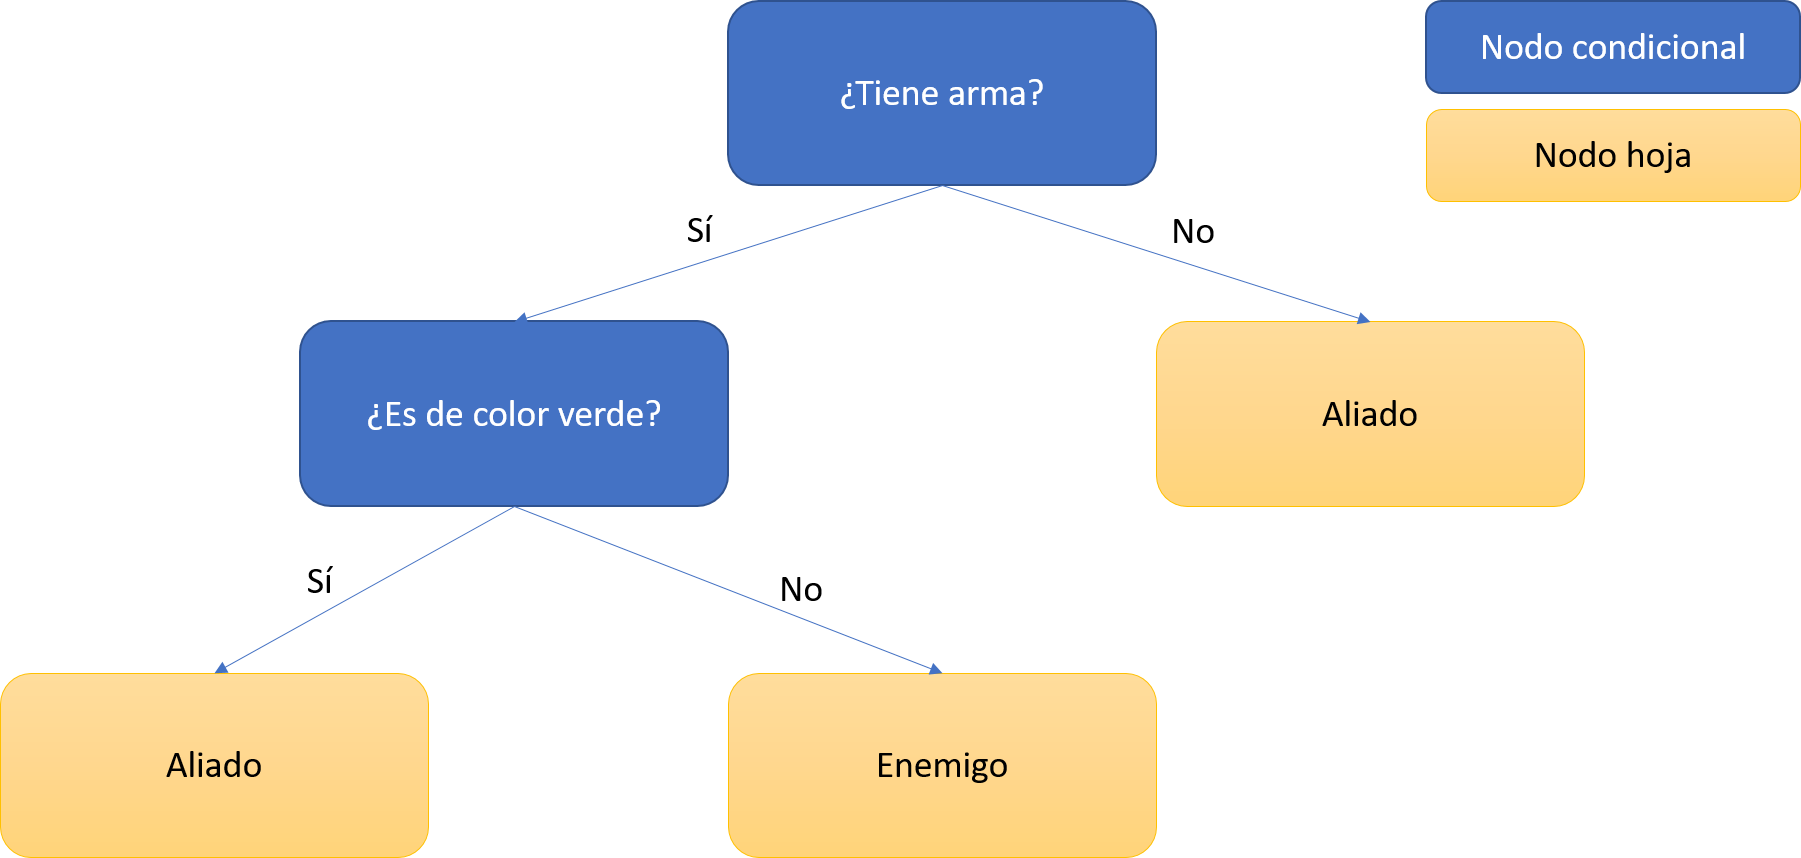
\includegraphics[width=\textwidth]{arbol-decision}
\caption{Árbol de decisión para determinar si un individuo es enemigo o aliado.}
\end{figure}

Los Árboles de Decisión suelen emplearse ampliamente en áreas donde sean necesarias decisiones deterministas automatizadas como finanzas, estadística, videojuegos, aprendizaje automático, etc. Son fáciles de entender y muy rápidos de procesar una vez construidos \cite{aihorizonDecisiontrees}.

En esta fase optamos por seguir un nuevo enfoque mediante Inteligencia Artificial Reactiva. Esto significa evaluar en cada turno un árbol de decisión (partiendo siempre desde la raíz), comprobando una serie de condiciones del estado de la partida, y a partir de ellas determinar una única acción a realizar. La decisión de seguir este enfoque persigue que nuestros bots resultantes tengan un comportamiento con continuidad dentro de una misma situación pero a la vez sean capaz de adaptarse a cambios repentinos en el estado del juego. 
 
Por ejemplo,a partir del código:
\begin{lstlisting}[caption=Ejemplo de código]
    if ( getDistanceToClosestNonEdibleGhost >= 4 ){
        getDirectionToClosestEdibleGhost
    } else {
        getDirectionAwayFromClosestNonEdibleGhost
    }
\end{lstlisting}

construiríamos el siguiente árbol:
\begin{figure}[H]
\centering
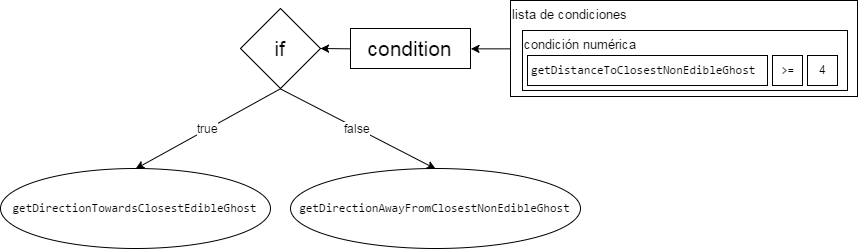
\includegraphics[width=\textwidth]{codigo-a-arbol}
\caption{Árbol contruido a partir de ejemplo de código.}
\end{figure}
La ejecución de este árbol consistiría en turno a turno evaluar desde el nodo raíz: primero, comprobar si la distancia al fantasma no comible más cercano es menor o igual que 4. En caso de que sea así, evalúa la rama izquierda recursivamente, y al ser esta un nodo hoja ejecuta la acción determinada por este, en este caso acercarse al fantasma comible más cercano. En caso de la que condición no se cumpla, se ejecutará de forma análoga la rama derecha, tratándose de un nodo hoja con la acción que genera un movimiento de huida del fantasma más cercano. 

\subsection{Árboles de decisión}
Posteriormente optamos por un cambio en la representación del fenotipo. Concretamente, a partir de cada fenotipo generado por el algoritmo evolutivo, generamos un árbol de decisión para simplificar significativamente la ejecución de una partida con dicho fenotipo, y así lograr la ya mencionada Inteligencia Artificial Reactiva. Dicho árbol contiene las diferentes funciones para consultar el estado de juego (los nodos no terminales) y para decidir movimientos (nodos terminales) como enumerados, obteniéndose cada movimiento evaluando recursivamente el árbol.
 
La razón de estos árboles era poder codificar comportamientos mucho más complejos en sus diferentes ``ramas'', pudiendo además explotar la riqueza de las gramáticas, simplificar la lógica de ejecución, y desarrollar una base mucho más estable sobre la que apoyar futuras iteraciones.

\subsection{Parsing de fenotipo a árbol}
A la hora de realizar el cambio estructural de fenotipo, optamos por realizar un parsing del fenotipo desde una cadena de caracteres (producida por JECO mediante evolución gramatical) a un árbol que organiza los ya mencionados condicionales, consecuentes y movimientos de la forma más intuitiva posible. La estructuración de dichos elementos dentro del árbol se realiza de la siguiente forma:

\subsubsection{Nodos terminales}
Los nodos terminales realizan una acción o una consulta. Si es una acción puede tratarse de:
\begin{itemize}
\item Movimientos simples (direccionales)
\item Movimientos basados en información del juego. Por ejemplo, ``el movimiento que aleja más a Pac-Man del fantasma más cercano''
\end{itemize}

En el caso de las consultas al estado del juego, estas pueden devolver distancias en formato entero (distancia al fantasma comible más cercano, ...) o booleanos (¿Está Pac-Man en una intersección?, ...).

\subsubsection{Nodos condicionales}
Los nodos condicionales contienen una lista de parámetros booleanos (los cuales hemos denominado condiciones) y otra lista que indica qué operadores booleanos binarios operan dichos parámetros. En caso de tratarse de un \texttt{if}, contendrá un nodo hijo con un consecuente, y en caso de ser un \texttt{else}, dos.
 
Una condición puede ser de varios tipos, según el tipo de los parámetros que contenga:
\begin{itemize}
\item de función booleana
\item de función numérica, operador numérico (binario) y función numérica
\item de función numérica, operador numérico (binario) y número
\item de número, operador numérico (binario) y función numérica
\end{itemize}

Los parámetros de tipo función que contenga una condición una vez más se trataran de enumerados, con la diferencia de que en este caso el método que poseen indicará el valor (booleano o numérico) de la consulta del estado de alguna variable de la partida. Finalmente, una condición puede encontrarse negada.

\subsection{Adaptador de árbol a movimiento de Pac-Man}
Para poder ejecutar partidas con estos árboles de decisión, necesitamos implementar un nuevo controlador de Pac-Man. Este controlador contiene el árbol de derivación, actuando como wrapper, de forma que con cada solicitud de movimiento realizada al controlador, este evalúa el árbol de forma recursiva, hasta encontrar un nodo terminal que devuelva un movimiento y que cumple todas sus condiciones previas.

Nótese  que la evaluación de dichos condicionales supone la evaluación de numerosos parámetros booleanos y enteros evaluados entre sí. Estos parámetros son obtenidos directamente de consultas al estado de la partida.

Finalmente se obtiene un movimiento, bien generado por la acción de un nodo terminal a través de la llamada a una determinada función interna del juego Ms. Pac-Man vs Ghosts, bien realizando un movimiento simple direccional.

\section{Gramáticas desarrolladas}
Todas nuestras gramáticas producen códigos basados en inteligencias artificiales reactivas, es decir, a cada turno de movimiento (denominado internamente como \textit{tick}) se evalúan una serie de condiciones del estado del tablero para producir un único movimiento de forma no ambigua. Las gramáticas diseñadas usan una estructura de anidamientos de declaraciones \texttt{if-else} que posteriormente un \textit{parser}\footnote{Un parser es una herramienta que mediante el uso de una gramática transforma texto escrito en el lenguaje representado por la gramática a una representación interpretable por otro sistema \cite{parserTechopedia}.
} convertirá a un Árbol de Decisión. Este Árbol de Decisión tendrá una traducción directa de las funciones escritas en la Gramática a funciones interpretables por el bot (escritas en \textit{Java}) que serán ejecutadas en el proceso de evaluación.
 
A la hora de desarrollar gramáticas las dividimos en tres categorías dependiendo del tipo de acciones que pueden producir:
\begin{itemize}
\item Bajo nivel: Son gramáticas cuyos nodos terminales, aquellos que dicen al bot de Pac-Man qué movimiento hacer en cada \textit{tick} del juego, se constituyen únicamente de las funciones \texttt{Up, Down, Left, Right} que son una codificación directa de las teclas de movimiento que dispondría un humano al jugar el juego.

\item Medio nivel: En lugar de las funciones básicas de movimiento (\texttt{Up, Down, ...}), disponen de funciones de un nivel medio,  entendiéndose nivel medio como funciones que dictan una acción directa, como puede ser comerse la \textit{pill} más cercana, huir del fantasma más cercano, ir a por la \textit{power pill} más cercana, etc.

\item Alto nivel: Se diferencian de las de medio nivel en que sus funciones terminales son muy abstractas y no se puede determinar directamente qué dirección o comportamiento tomará el bot, estas funciones son del estilo de \textit{comer, huir, atacar, ...} funciones que se entienden cuál es su objetivo pero que pueden realizarse de distintas maneras.
\end{itemize}

\subsection{Parámetros del experimento realizado} \label{sec:params}
Todos los resultados de esta sección han sido obtenidos empleando los mismos operadores, parámetros y probabilidad con la que se emplean los operadores del algoritmo evolutivo para permitir una comparación objetiva del rendimiento empleando diferentes gramáticas. Estos parámetros son:
\begin{table}[H]
\centering
\begin{tabular}{lc|c|}
\cline{3-3}
\textbf{}                                                                & \multicolumn{1}{l|}{\textbf{}}     & \multicolumn{1}{l|}{\textbf{Porcentaje}} \\ \hline
\multicolumn{1}{|l|}{\textbf{Población}}                                 & 100                                & -                                        \\ \hline
\multicolumn{1}{|l|}{\textbf{Generaciones}}                              & 100                                & -                                        \\ \hline
\multicolumn{1}{|l|}{\textbf{Evaluaciones por individuo}}                & 30                                 & -                                        \\ \hline
\multicolumn{1}{|l|}{\textbf{Longitud cromosoma}}                        & 100                                & -                                        \\ \hline
\multicolumn{1}{|l|}{\textbf{Límite superior codón\footnotemark[2]}} & 256                                & -                                        \\ \hline
\multicolumn{1}{|l|}{\textbf{Método de selección}}                       & Torneo Binario\footnotemark[3] & -                                        \\ \hline
\multicolumn{1}{|l|}{\textbf{Método de cruce}}                           & LHS                                & 60                                       \\ \hline
\multicolumn{1}{|l|}{\textbf{Método de mutación}}                        & Integer Flip                       & 10                                       \\ \hline
\multicolumn{1}{|l|}{\textbf{Mutación Neutral}}                          & Sí                                 & -                                        \\ \hline
\multicolumn{1}{|l|}{\textbf{Elitismo}}                                  & Sí                                 & 5                                        \\ \hline
\end{tabular}
\caption{Parámetros utilizados.}
\end{table}
\footnotetext[2]{valor máximo que puede tomar}
\footnotetext[3]{o NSGA II si se está empleando multiobjetivo}

\subsection{Gramática de bajo nivel}
Con la gramática de bajo nivel pretendemos que el bot tenga un comportamiento basado en estímulos muy específicos y utilizando solo los operadores de movimiento de los que un jugador humano dispone (\texttt{moveup, moveDown, moveRight, moveLeft}). Como son operadores de bajo nivel que no disponen de información del juego (\textit{pill} más cercana, posición de fantasmas, etc), la gramática necesita contener una gran cantidad de funciones que devuelvan información del estado actual del juego:
\begin{itemize}
\item \texttt{getDistanceToClosestNonEdibleGhost}: Devuelve la distancia al fantasma peligroso más cercano.

\item \texttt{getDistanceToClosestNonEdibleGhost{Up, Down, Left, Right}}: Distancia al fantasma peligroso más cercano a la posición del bot en la dirección dada.

\item \texttt{getDistanceToClosestEdibleGhost}: Devuelve la distancia al fantasma comestible más cercano.

\item \texttt{getDistanceToClosestEdibleGhost{Up, Down, Left, Right}}: Distancia al fantasma comestible más cercano a la posición del bot en la dirección dada.

\item \texttt{getNumberOfActivePowerPills}: Devuelve la cantidad de \textit{power pills} que se encuentran actualmente en el tablero.

\item \texttt{getDistanceToClosestPill}: Distancia a la \textit{pill} (también considerando las \textit{power pills}) más cercana independientemente de la orientación del bot.

\item \texttt{getDistanceToClosestPill{Up, Down, Left Right}}: Devuelve la \textit{pill} más cercana al bot en la dirección especificada.

\item \texttt{getClosesPowerPill{Up, Down, Left Right}}: Idéntica a las anteriores pero teniendo en cuenta solo las \textit{power pills}.

\item \texttt{getClosestJunctionExitsNumber{Up, Down, Left, Right}} = Número de salidas de la intersección más cercana a la posición del bot en la dirección dada.

\item \texttt{getDistanceToClosestJunction{Up, Down, Left, Right}} = Distancia del bot a la intersección más cercana dada una dirección.

\item \texttt{getClosestNonEdibleGhostDistanceToClosestJunction{Up, Down, Left Right}}: Devuelve la distancia del fantasma peligroso más cercano a la intersección más cercana al bot en la dirección dada.

\item \texttt{getClosestEdibleGhostDistanceToClosestJunction{Up, Down, Left Right}}: Identica a las anteriores funciones pero con fantasmas comestibles.

\item \texttt{getGeometricMeanDistanceToNonEdibleGhosts}: Devuelve la distancia media geométrica a los fantasmas peligrosos.

\item \texttt{getGeometricMeanDistanceToEdibleGhosts}: Idéntica a la anterior pero la distancia a los fantasmas comestibles.
\end{itemize}

Los resultados de estos operadores de obtención del estado del juego se comparan dentro de las condiciones de las declaraciones \texttt{if} contra un número. Este número en vez de permitir generarlo de forma arbitraria por la gramática lo que hemos decidido es introducir nosotros un conjunto discreto de números que pueden ser escogidos para las comparaciones, reduciendo de este modo el espacio de búsqueda y la generaciones de números absurdos (extremadamente grandes).

\subsubsection{Notación BNF}
\begin{lstlisting}[caption={Gramática de bajo nivel.}]
<grammar> ::= <selection-statement>
 
<selection-statement> ::= if( <condition> ){ <statement> }
                          else{ <statement> }
                        | if( <condition> ){ <statement> }
 
<statement> ::= <terminal-func>
              | <selection-statement>
 
<terminal-func> ::= <simpleMoves>
 
<condition> ::= <number-func> <number-operator> <number>
 
<number-func> ::= getDistanceToClosestNonEdibleGhost
                | getDistanceToClosestNonEdibleGhostUp
                | getDistanceToClosestNonEdibleGhostDown
                | ... 
 
<number-operator> ::= ==
                    | !=
                    | <
                    | >
                    | <=
                    | >=
 
<simpleMoves> ::= moveUp
                | moveDown
                | moveLeft
                | moveRight
 
<number> ::=  5 | 10 | 15 | 20 | 25 | 30
           | 40 | 50 | 60 | 75 | 80 | 90
\end{lstlisting}

\subsubsection{Resultados}
\begin{figure}[H]
\centering
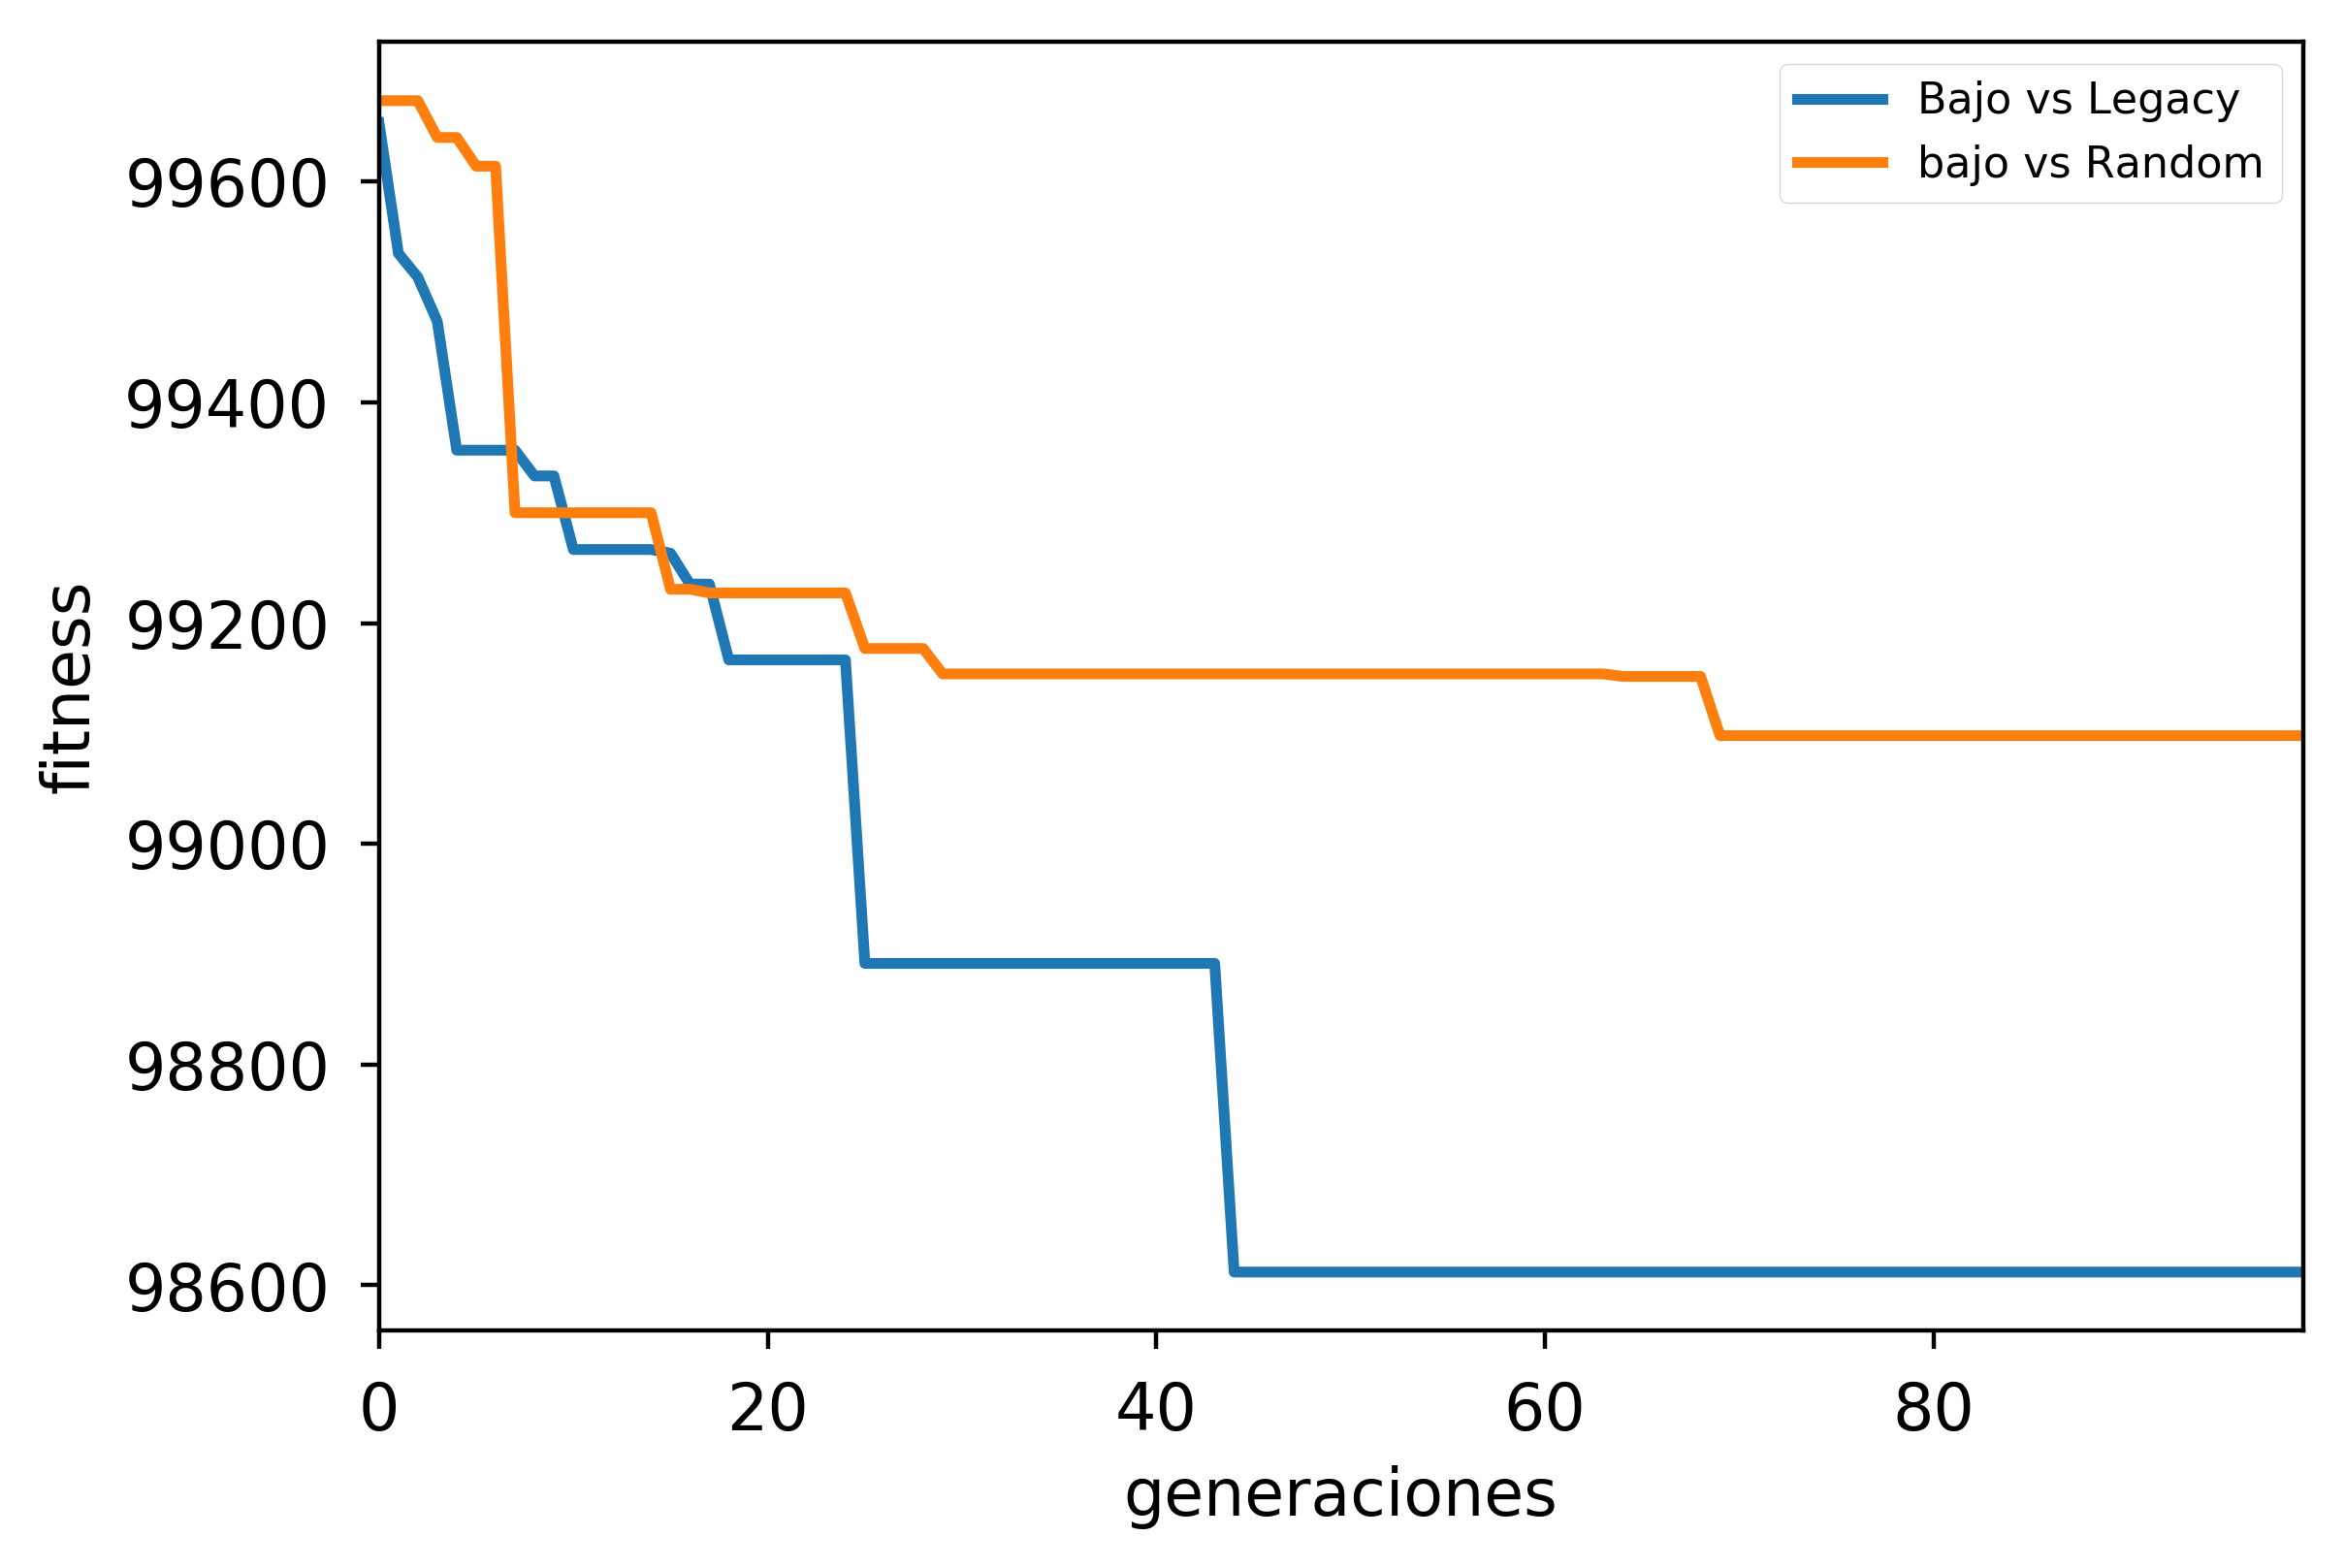
\includegraphics[width=0.8\textwidth]{grafica/low_level}
\caption{Gráfica que muestra las primeras 100 generaciones de dos ejecuciones distintas contra los controladores de fantasmas Random y Legacy usando la gramática de bajo nivel. Función fitness: 1000000 - puntos obtenidos.}
\end{figure}

Se obtuvieron las siguientes conclusiones a través de distintas ejecuciones:
\begin{itemize}
\item Los programas generados (fenotipo) son bastante largos debido a que hay muchos anidamientos de \texttt{if-else} que generan distintas acciones para determinados casos particulares. Esto es un resultado esperado al usar la gramática de bajo nivel.

\item Se obtienen malos resultados en cuanto a puntos obtenidos pero hay una gran convergencia de la población hacia el individuo óptimo actual.

\item El comportamiento del mejor individuo es siempre el mismo. Pac-Man va directamente a la esquina inferior izquierda del nivel y se queda quieto en cierto punto en el cual los fantasmas no le detectan, consiguiendo pasarse niveles porque el juego cada 4000 \textit{ticks} cambia de nivel inexorablemente y da una cierta cantidad de puntos al jugador. Este error del juego solo lo detecta hasta el nivel 3, nivel en el que es siempre eliminado por los fantasmas. A este comportamiento le hemos denominado bot ``Camper''.
\end{itemize}

\begin{lstlisting}[caption={Ejemplo de bot típico producido usando la gramática de bajo nivel entrenado contra Random Ghosts.}]
if (getDistanceToClosestNonEdibleGhostUp != 25) {
  if (getDistanceToClosestNonEdibleGhostLeft <= 90) {
    moveRight
  } else {
    if (getDistanceToClosestJunctionLeft <= 10) {
      if (getClosestEdibleGhostDistanceToClosestJunctionRight < 20) {
        if (getDistToClosestPowerPillUp < 30) {
          moveLeft
        } else {
          if (getDistanceToClosestNonEdibleGhostDown > 25) {
            moveRight
          } else {
            moveRight
          }
        }
      } else {
        if (getGeometricMeanDistanceToNonEdibleGhosts < 10) {
          moveLeft
        } else {
          if (getClosestJunctionExitsNumberLeft > 20) {
            if (getNumberOfActivePowerPills > 90) {
              if (getClosestJunctionExitsNumberUp != 10) {
                moveLeft
              }
            }
          } else {
            moveUp
          }
        }
      }
    } else {
      if (getDistToClosestPowerPillDown != 15) {
        moveUp
      } else {
        if (getDistanceToClosestNonEdibleGhostUp > 60) {
          if (getClosestEdibleGhostDistanceToClosestJunctionRight < 60) {
            if (getDistToClosestPowerPillLeft > 5) {
              if (getNumberOfActivePowerPills <= 25) {
                if (getDistanceToClosestEdibleGhost > 25) {
                  moveLeft
                } else {
                  if (getDistanceToClosestEdibleGhost >= 5) {
                    if (getClosestEdibleGhostDistanceToClosestJunctionRight > 10) {
                      if (getDistToClosestPowerPillUp >= 50) {
                        moveRight
                      } else {
                        if (getDistanceToClosestJunctionUp == 75) {
                          moveUp
                        } else {
                          if (getClosestJunctionExitsNumberLeft == 20) {
                            moveDown
                          }
                        }
                      }
                    } else {
                      moveDown
                    }
                  } else {
                    moveDown
                  }
                }
              } else {
                moveUp
              }
            } else {
              moveUp
            }
          }
        }
      }
    }
  }
} else {
  if (getClosestEdibleGhostDistanceToClosestJunctionUp > 60) {
    if (getDistToClosestPowerPillLeft >= 40) {
      moveDown
    } else {
      moveUp
    }
  } else {
    moveLeft
  }
}
\end{lstlisting}

\begin{lstlisting}[caption={Mejor individuo producido usando la gramática de bajo nivel evolucionado jugando contra Legacy Ghosts.}]
    if (getDistanceToClosestNonEdibleGhostRight <= 5) {
        moveDown
    }
    else {
        if (getDistanceToClosestEdibleGhostLeft <= 40) {
            moveUp
        }
        else {
            moveRight
        }
    }
\end{lstlisting}

\subsection{Gramática de medio nivel}
Con esta gramática de medio nivel intentamos obtener mejores resultados en puntos que los obtenidos con la gramática de bajo nivel. Hemos eliminado de la gramática los operadores de movimientos básicos (\texttt{moveUp, moveDown, ...}) debido a que han sido sustituidos por operadores más abstractos y de más alto nivel:
\begin{itemize}
\item \texttt{getDirectionTowardsClosestPill}: Devuelve el movimiento a efectuar (arriba, abajo, derecha, izquierda) para ir hacia la \textit{pill} más cercana al bot.

\item \texttt{getDirectionAwayFromClosestNonEdibleGhost}: Devuelve el movimiento a efectuar para alejarse (normalmente en dirección contraria al fantasma) del fantasma peligroso más cercano.

\item \texttt{getDirectionTowardsClosestEdibleGhost}: Devuelve el movimiento hacia el fantasma comestible más cercano.

\item \texttt{getDirectionTowardsClosestPowerPill}: Devuelve el movimiento hacia la \textit{power pill} más cercana.
\end{itemize}

Dado que estos operadores de acción disponen internamente de acceso al estado del juego hemos optado por prescindir de los operadores de obtención de información menos utilizados o que no son útiles en la gramática de medio nivel (como la distancia a la \textit{pill} más cercana al bot en dirección arriba). De este modo solo dispone de los operadores más útiles (y los que prácticamente siempre usa) y permite guiar la búsqueda más eficientemente.

\subsubsection{Notación BNF}
\begin{lstlisting}[caption={Gramática de medio nivel.}]
<grammar> ::= <selection-statement>

<selection-statement> ::= if( <condition> ){ <statement> }
                          else{ <statement> }
                        | if( <condition> ){ <statement> }

<statement> ::= <terminal-func>
              | <selection-statement>

<terminal-func> ::= getDirectionTowardsClosestPill
                  | getDirectionAwayFromClosestNonEdibleGhost
                  | getDirectionTowardsClosestEdibleGhost
                  | getDirectionTowardsClosestPowerPill
                  
<condition> ::= <number-func> <number-operator> <number>

<number-func> ::= getDistanceToClosestNonEdibleGhost
                | getDistanceToClosestEdibleGhost
                | getNumberOfActivePowerPills
                | getDistToClosestPill
                | getDistToClosestPowerPill
                | getGeometricMeanDistanceToNonEdibleGhosts
                | getGeometricMeanDistanceToEdibleGhosts

<number-operator> ::= ==
                    | !=
                    | <
                    | >
                    | <=
                    | >=

<number> ::=  5 | 10 | 15 | 20 | 25 | 30
           | 40 | 50 | 60 | 75 | 80 | 90
\end{lstlisting}

\subsubsection{Resultados}
\begin{figure}[H]
\centering
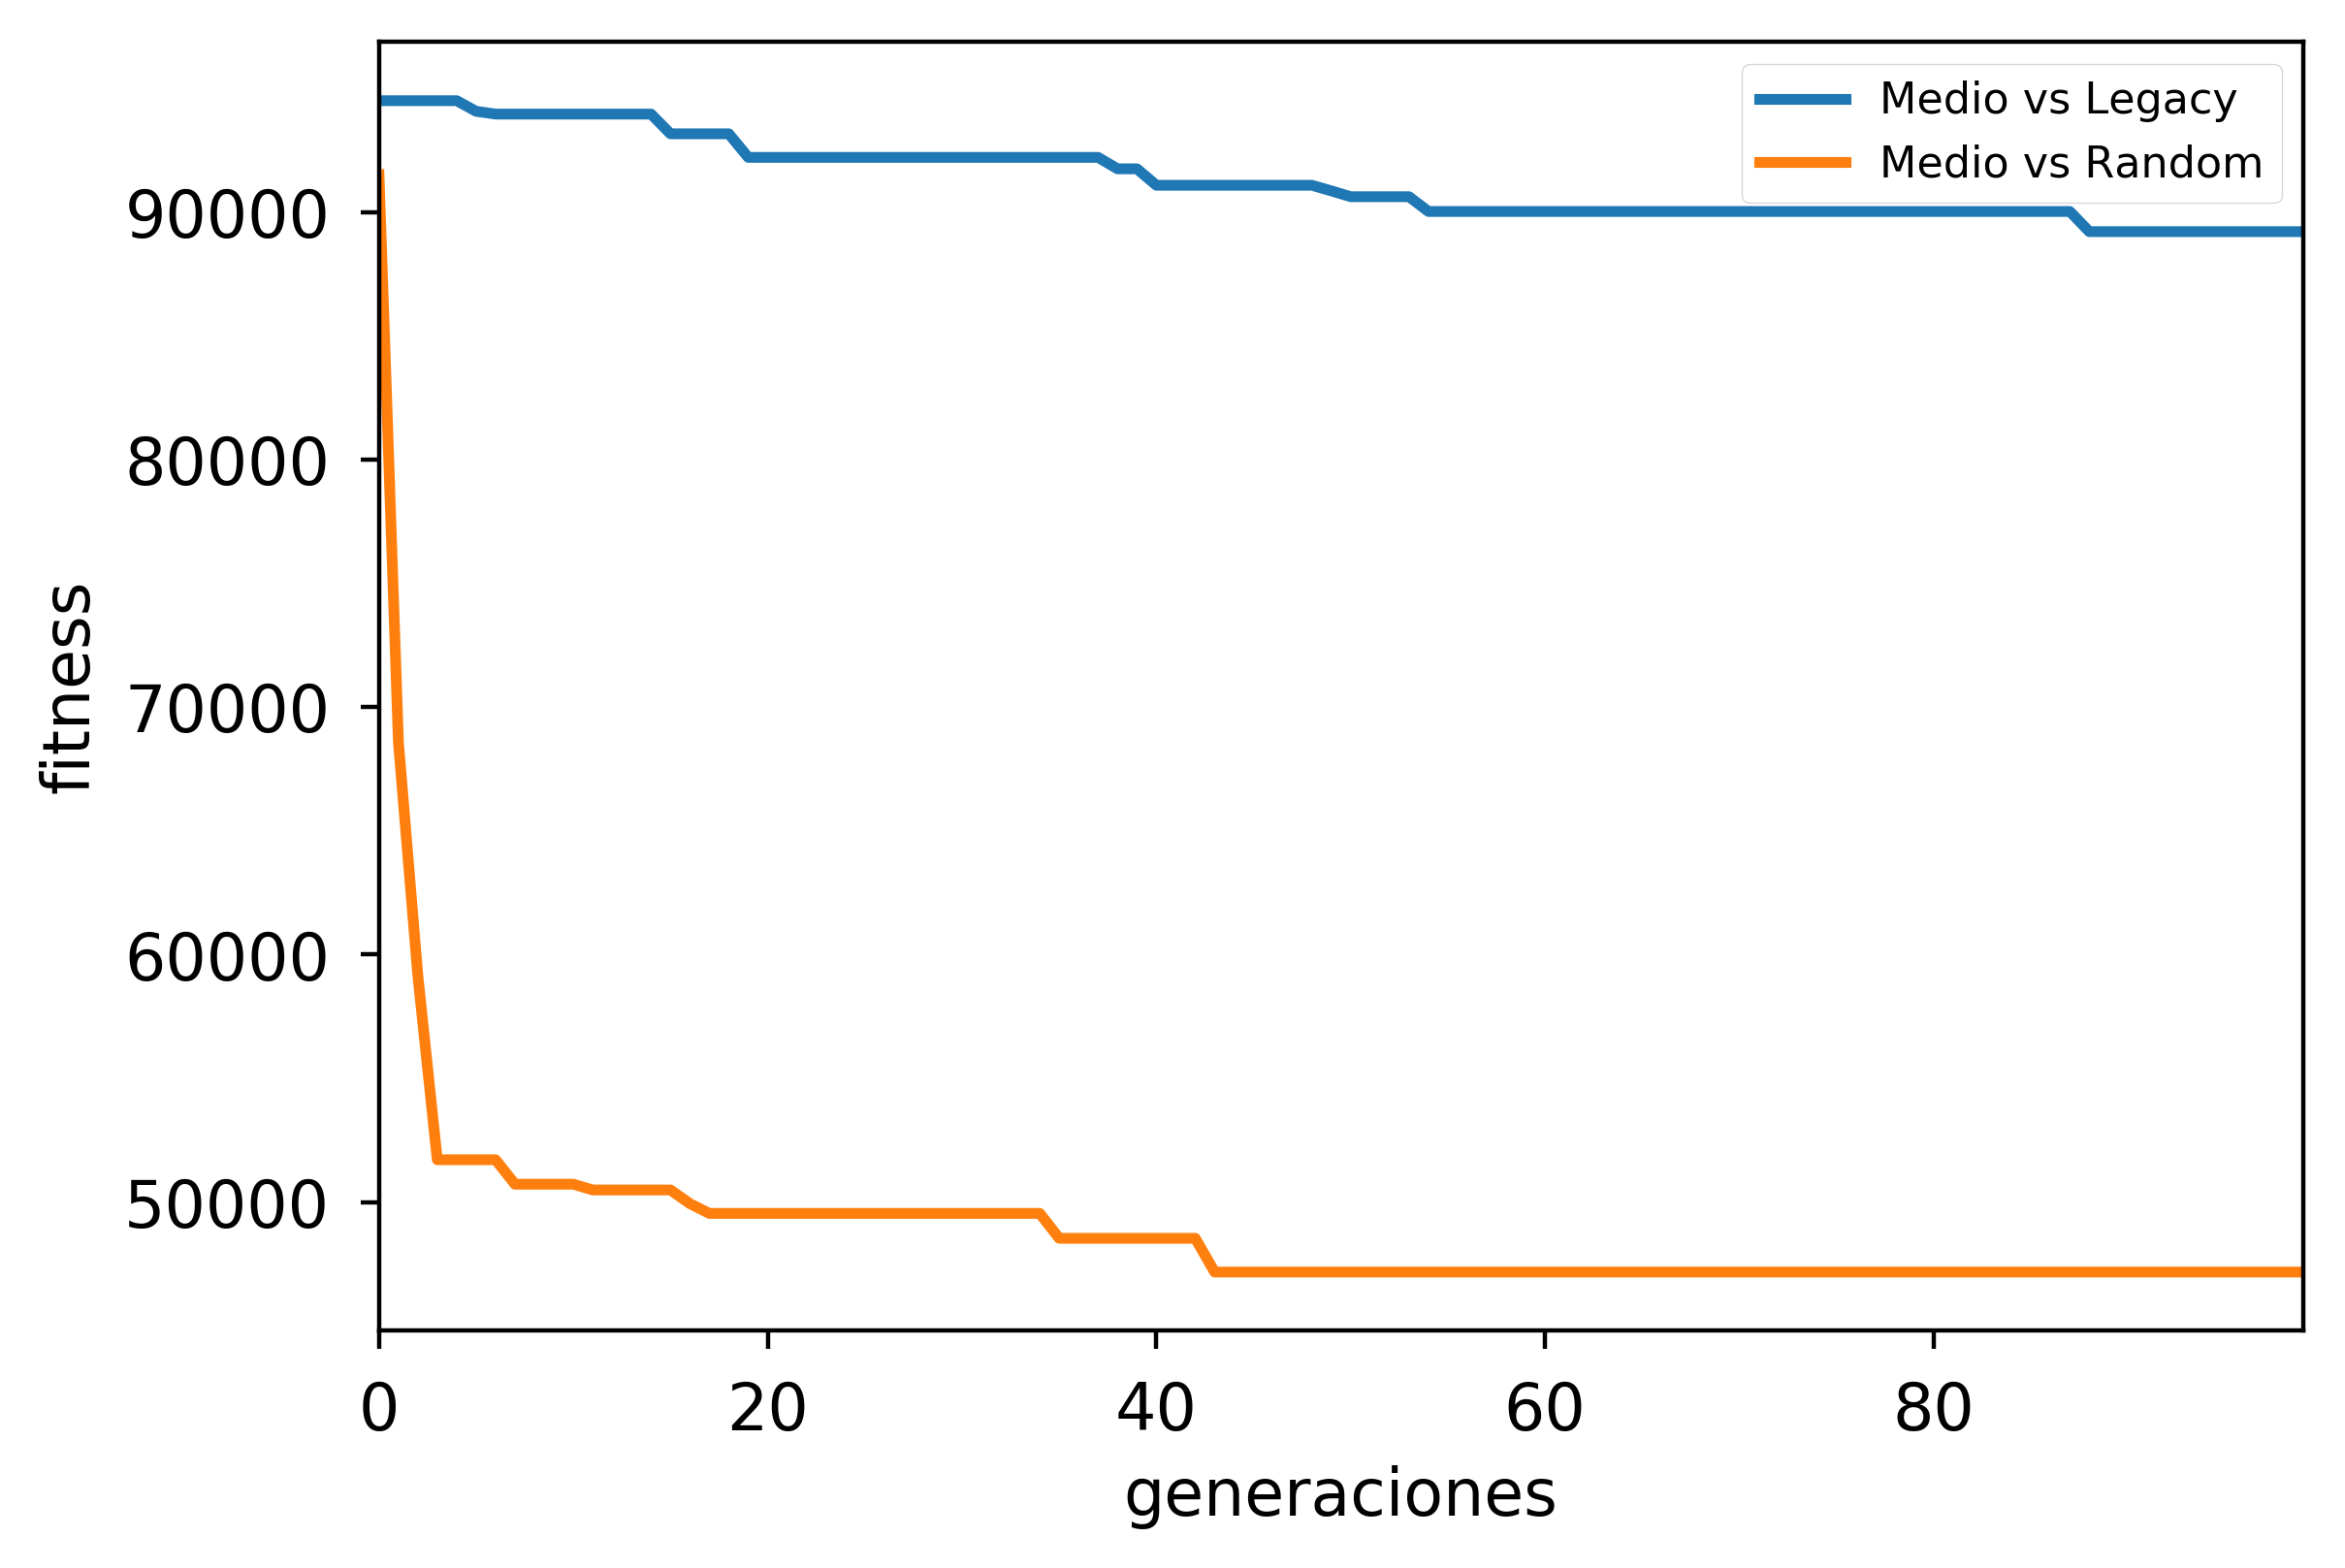
\includegraphics[width=0.8\textwidth]{grafica/medium_level}
\caption{Gráfica que muestra las primeras 100 generaciones de dos ejecuciones distintas contra los controladores de fantasmas Random y Legacy usando la gramática de medio nivel. Función fitness: 1000000 - puntos obtenidos.}
\end{figure}

Las conclusiones obtenidas son:
\begin{itemize}
\item La velocidad de ejecución del algoritmo evolutivo ha sido significativamente más rápida que la de bajo nivel, de forma que la ejecución se realiza en apenas unos minutos.

\item Los resultados obtenidos en puntos son bastante superiores a los obtenidos con la gramática de bajo nivel.

\item El código generado por el mejor individuo (fenotipo) es muy corto, generalmente consiste de un solo \textit{if-else} que contiene cada uno una única función.

\item Creemos que la longitud del código está directamente relacionada al comportamiento que poseen los mejores individuos y que es obtenido de forma recurrente. Al principio y si no hay fantasmas cercanos el bot solo realiza movimientos neutros (continuar en la misma dirección), quedándose atascado en una esquina del mismo modo que lo hace el bot ``Camper'' de la gramática de nivel bajo. Pero si un fantasma se acerca lo suficiente el bot pasa a un modo agresivo dirigiéndose a la \textit{power pill} más cercana, comiéndosela y cazando a tantos fantasmas como puede. Este comportamiento lo repite con todas las \textit{power pills} hasta que se queda sin ellas, pasando a un estado de movimiento neutral y siendo eliminado por los fantasmas sin pasar nunca del primer nivel del juego. Este comportamiento es debido a una característica del juego que provoca una explosión en la puntuación al comer fantasmas seguidos. Esto se debe a que durante el tiempo que dura el efecto de una \textit{power pill} cada fantasma comido da una serie de puntos, este valor es duplicado si se come otro fantasma y el nuevo valor es a su vez duplicado si otro fantasma es consumido. Esto permite obtener una gran cantidad de puntos provocando que el fitness de ese individuo destaque
\end{itemize}

Como se puede apreciar, la gramática de bajo nivel siempre lleva a un comportamiento de bot ``Camper'' y la gramática de medio nivel a un comportamiento de bot ``Cazador''. Estos comportamientos vienen dados principalmente por los puntos que se obtienen al jugar, por lo que investigamos el uso de una gramática de alto nivel y comparamos los resultados obtenidos con la gramática de medio nivel. Así mismo estudiamos distintas funciones \textit{fitness} y comprobamos si con estas nuevas funciones conseguimos mejores comportamientos.

\begin{lstlisting}[caption={Mejor individuo producido usando la gramática de medio nivel para evolucionar contra Random Ghosts.}]
    if (getDistanceToClosestNonEdibleGhost > 10) {
        if (getDistanceToClosestNonEdibleGhost < 20) {
            getDirectionTowardsClosestPowerPill 
        }
        else {
            getDirectionTowardsClosestPill
        }
    }
    else {
        getDirectionAwayFromClosestNonEdibleGhost
    }
\end{lstlisting}

\begin{lstlisting}[caption={Mejor individuo producido usando la gramática de medio nivel para evolucionar contra Legacy Ghosts.}]
    if (getDistanceToClosestNonEdibleGhost >= 5) {
        getDirectionTowardsClosestPill
    } else {
        getDirectionAwayFromClosestNonEdibleGhost
    }
\end{lstlisting}

\subsection{Gramática de alto nivel}
Tras los resultados obtenidos con las gramáticas anteriores, decidimos estudiar hasta qué punto sería posible mejorarlos mediante el empleo de una gramática de alto nivel, empleando  un número reducido de funciones de alto nivel, proporcionándole de esta forma conocimiento experto.

\subsubsection{Nuevas funciones de alto nivel}

\paragraph{escapeHL}
Genera un movimiento de huida hacia la \textit{power pill} mas cercana si puede alcanzarla antes que el fantasma más cercano. Si no llega a tiempo o bien no quedan \textit{power pill}s, genera un movimiento de huida del fantasma más cercano en la dirección que más le aleje de él.

\paragraph{attackHL}
Genera un movimiento hacia el fantasma más comible cercano siempre que este pueda ser alcanzado por otro fantasma no comible antes. Si no hay fantasmas comibles, genera un movimiento igual a la última dirección en la que se movió.

\paragraph{seekFoodHL}
Genera un movimiento hacia la \textit{pill} más cercana (o si no quedan \textit{pills}, la \textit{power pill} más cercana) siempre y cuando sea alcanzable por Pac-Man antes que por un fantasma. Si no llega a tiempo, mueve en la última dirección en la que lo hizo el turno anterior.

\subsubsection{Notación BNF}
\begin{lstlisting}[caption={Gramática de alto nivel.}]
<grammar> ::= <selection-statement>

<selection-statement> ::= if( <condition> ){ <statement> }
                          else{ <statement> }
                        | if( <condition> ){ <statement> }

<statement> ::= <terminal-func>
              | <selection-statement>

<terminal-func> ::= escapeHL
                  | attackHL
                  | seekFoodHL

<condition> ::= <number-func> <number-operator> <number>

<number-func> ::= getDistanceToClosestNonEdibleGhost
                | getDistanceToClosestEdibleGhost

<number-operator> ::= ==
                    | !=
                    | <
                    | >
                    | <=
                    | >=

<number> ::=  5 | 10 | 15 | 20 | 25 | 30
           | 40 | 50 | 60 | 75 | 80 | 90
\end{lstlisting}

\subsubsection{Resultados}
Debido al conocimiento experto que poseen las funciones, la gramática utilizada solo contiene como operadores de acción las tres funciones de alto nivel comentadas, dos operadores de obtención de información del tablero  (\texttt{getDistanceToClosestNonEdibleGhost} y \texttt{getDistanceToClosestEdibleGhost}) debido a que recurrentemente han sido las más utilizadas, el comportamiento de los mejores bots obtenidos con las gramáticas anteriores se basan únicamente en ellas para la toma de decisiones.
\begin{figure}[H]
\centering
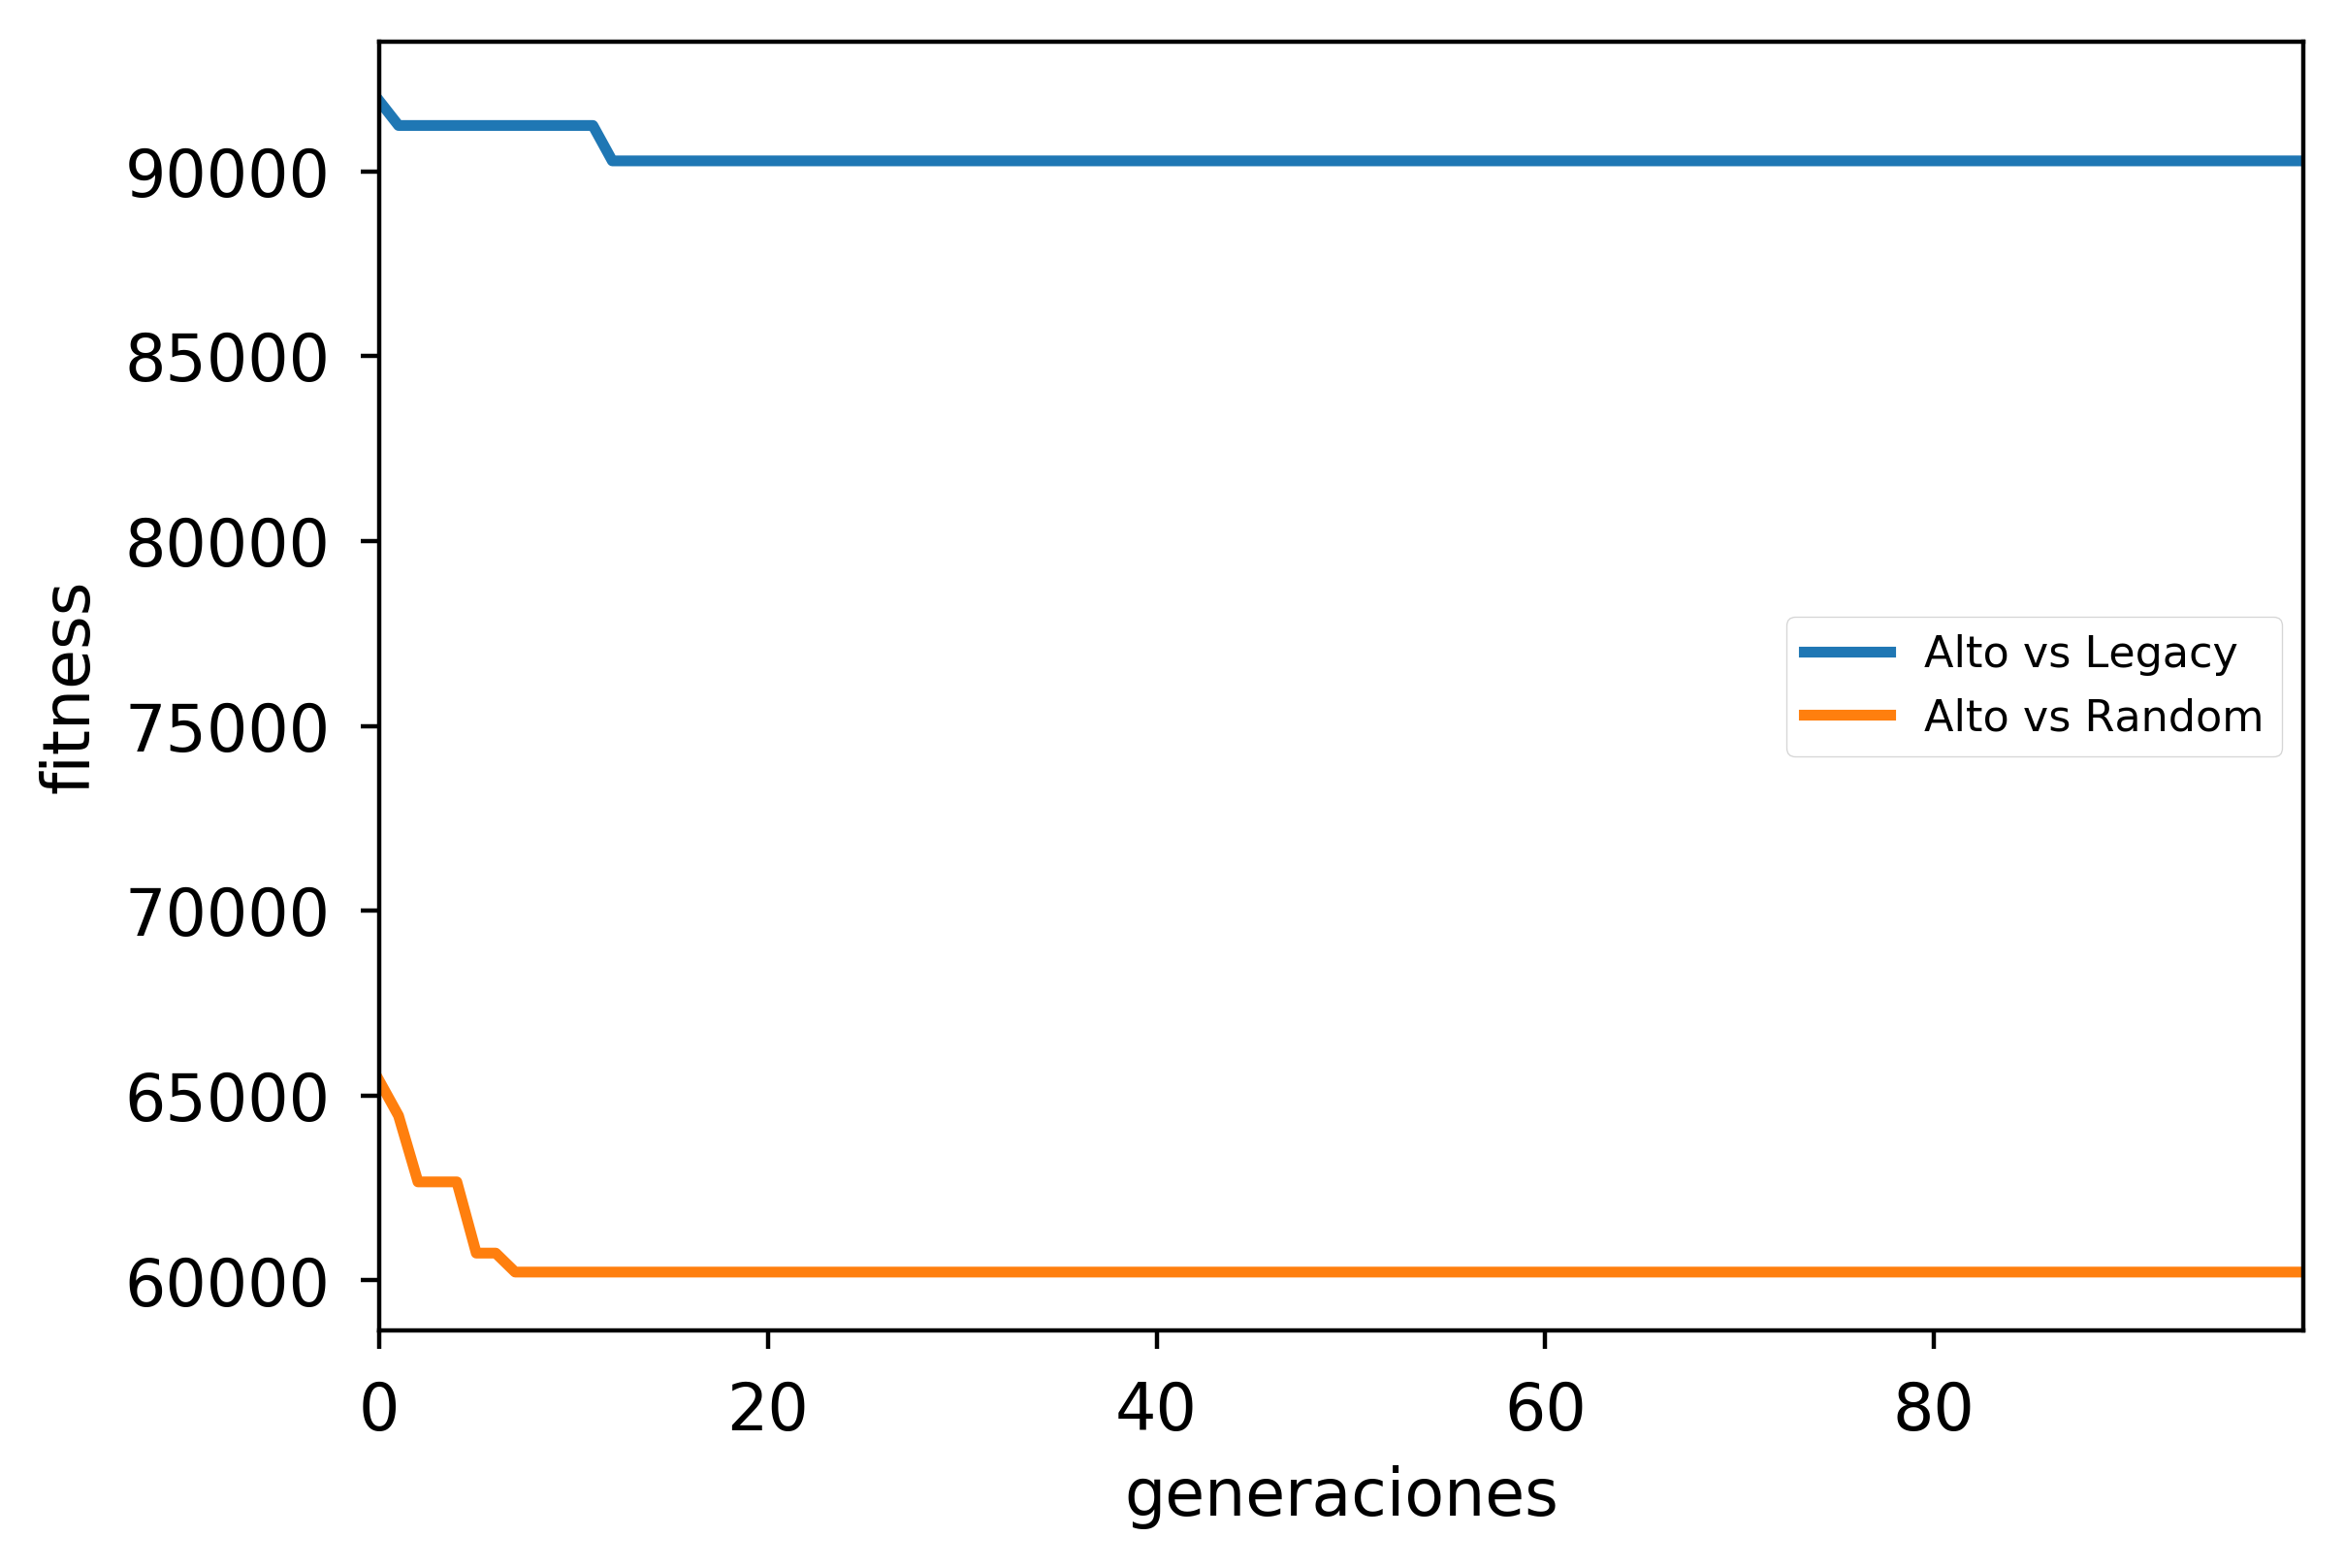
\includegraphics[width=0.8\textwidth]{grafica/high_level}
\caption{Gráfica que muestra las primeras 100 generaciones de dos ejecuciones distintas contra los controladores de fantasmas Random y Legacy usando la gramática de alto nivel. Función \textit{fitness}: $1000000 - puntos obtenidos$.}
\end{figure}

Las conclusiones obtenidas al evolucionar el bot usando esta gramática fueron:
\begin{itemize}
\item La velocidad de ejecución del algoritmo es aún más rápida que con la gramática de medio nivel, de forma que la ejecución se realiza en apenas unos segundos.

\item El código generado habitualmente se parece mucho al obtenido mediante la gramática de medio nivel: Un \textit{if-else} con una inecuación numérica que generalmente tiene en cuenta el fantasma más cercano. La más notable diferencia es que las acciones de medio nivel como \texttt{getDirectionAwayFromClosestNonEdibleGhost}, se ven sustituidas por su correspondiente directa de alto nivel, como \texttt{escapeHL}.
\begin{lstlisting}[caption={Código del mejor individuo obtenido en una población evolucionada con la gramática de medio nivel.}]
    if (getDistanceToClosestNonEdibleGhost >= 5) {
        getDirectionTowardsClosestPill
    } else {
        getDirectionAwayFromClosestNonEdibleGhost
    }
\end{lstlisting}

\begin{lstlisting}[caption={Código del mejor individuo obtenido en una población evolucionada con la gramática de alto nivel.}]
    if (getDistanceToClosestNonEdibleGhost <= 5) {
        escapeHL
    } else {
        seekFoodHL
    }
\end{lstlisting}

\item Obtiene buenos resultados muy rápidamente comparada con la gramática de medio nivel (Figura~\ref{grafica:comparacion-todas}). Esto se debe probablemente al reducido espacio de búsqueda de soluciones al ser una gramática tan compacta. Sin embargo y como se analizó en nuestro artículo (Apartado~\ref{cap:paper}),  la evolución utilizando la gramática de alto nivel se estanca en un óptimo local y es superada por la de medio nivel que obtiene mejores resultados, como se puede apreciar en la Figura~\ref{grafica:comparacion-todas}. La de medio nivel consigue algunos puntos más en promedio con 100 generaciones.
\end{itemize}

Todo esto nos indica que para tareas en las que es importante obtener buenos resultados de forma rápida, conviene favorecer gramáticas de alto nivel, mientras que si buscamos los mejores resultados posibles a cambio de un tiempo de evolución largo, conviene usar gramáticas de medio nivel.

\begin{lstlisting}[caption={Ejemplo de bot producido al evolucionar usando la gramática de alto nivel (mismo resultado entrenando tanto contra Random Ghosts como Legacy Ghosts).}]
    if (getDistanceToClosestNonEdibleGhost <= 5) {
        escapeHL
    } else {
        seekFoodHL
    }
\end{lstlisting}

\subsection{Comparativa gráfica de niveles}
\begin{figure}[H]
\centering
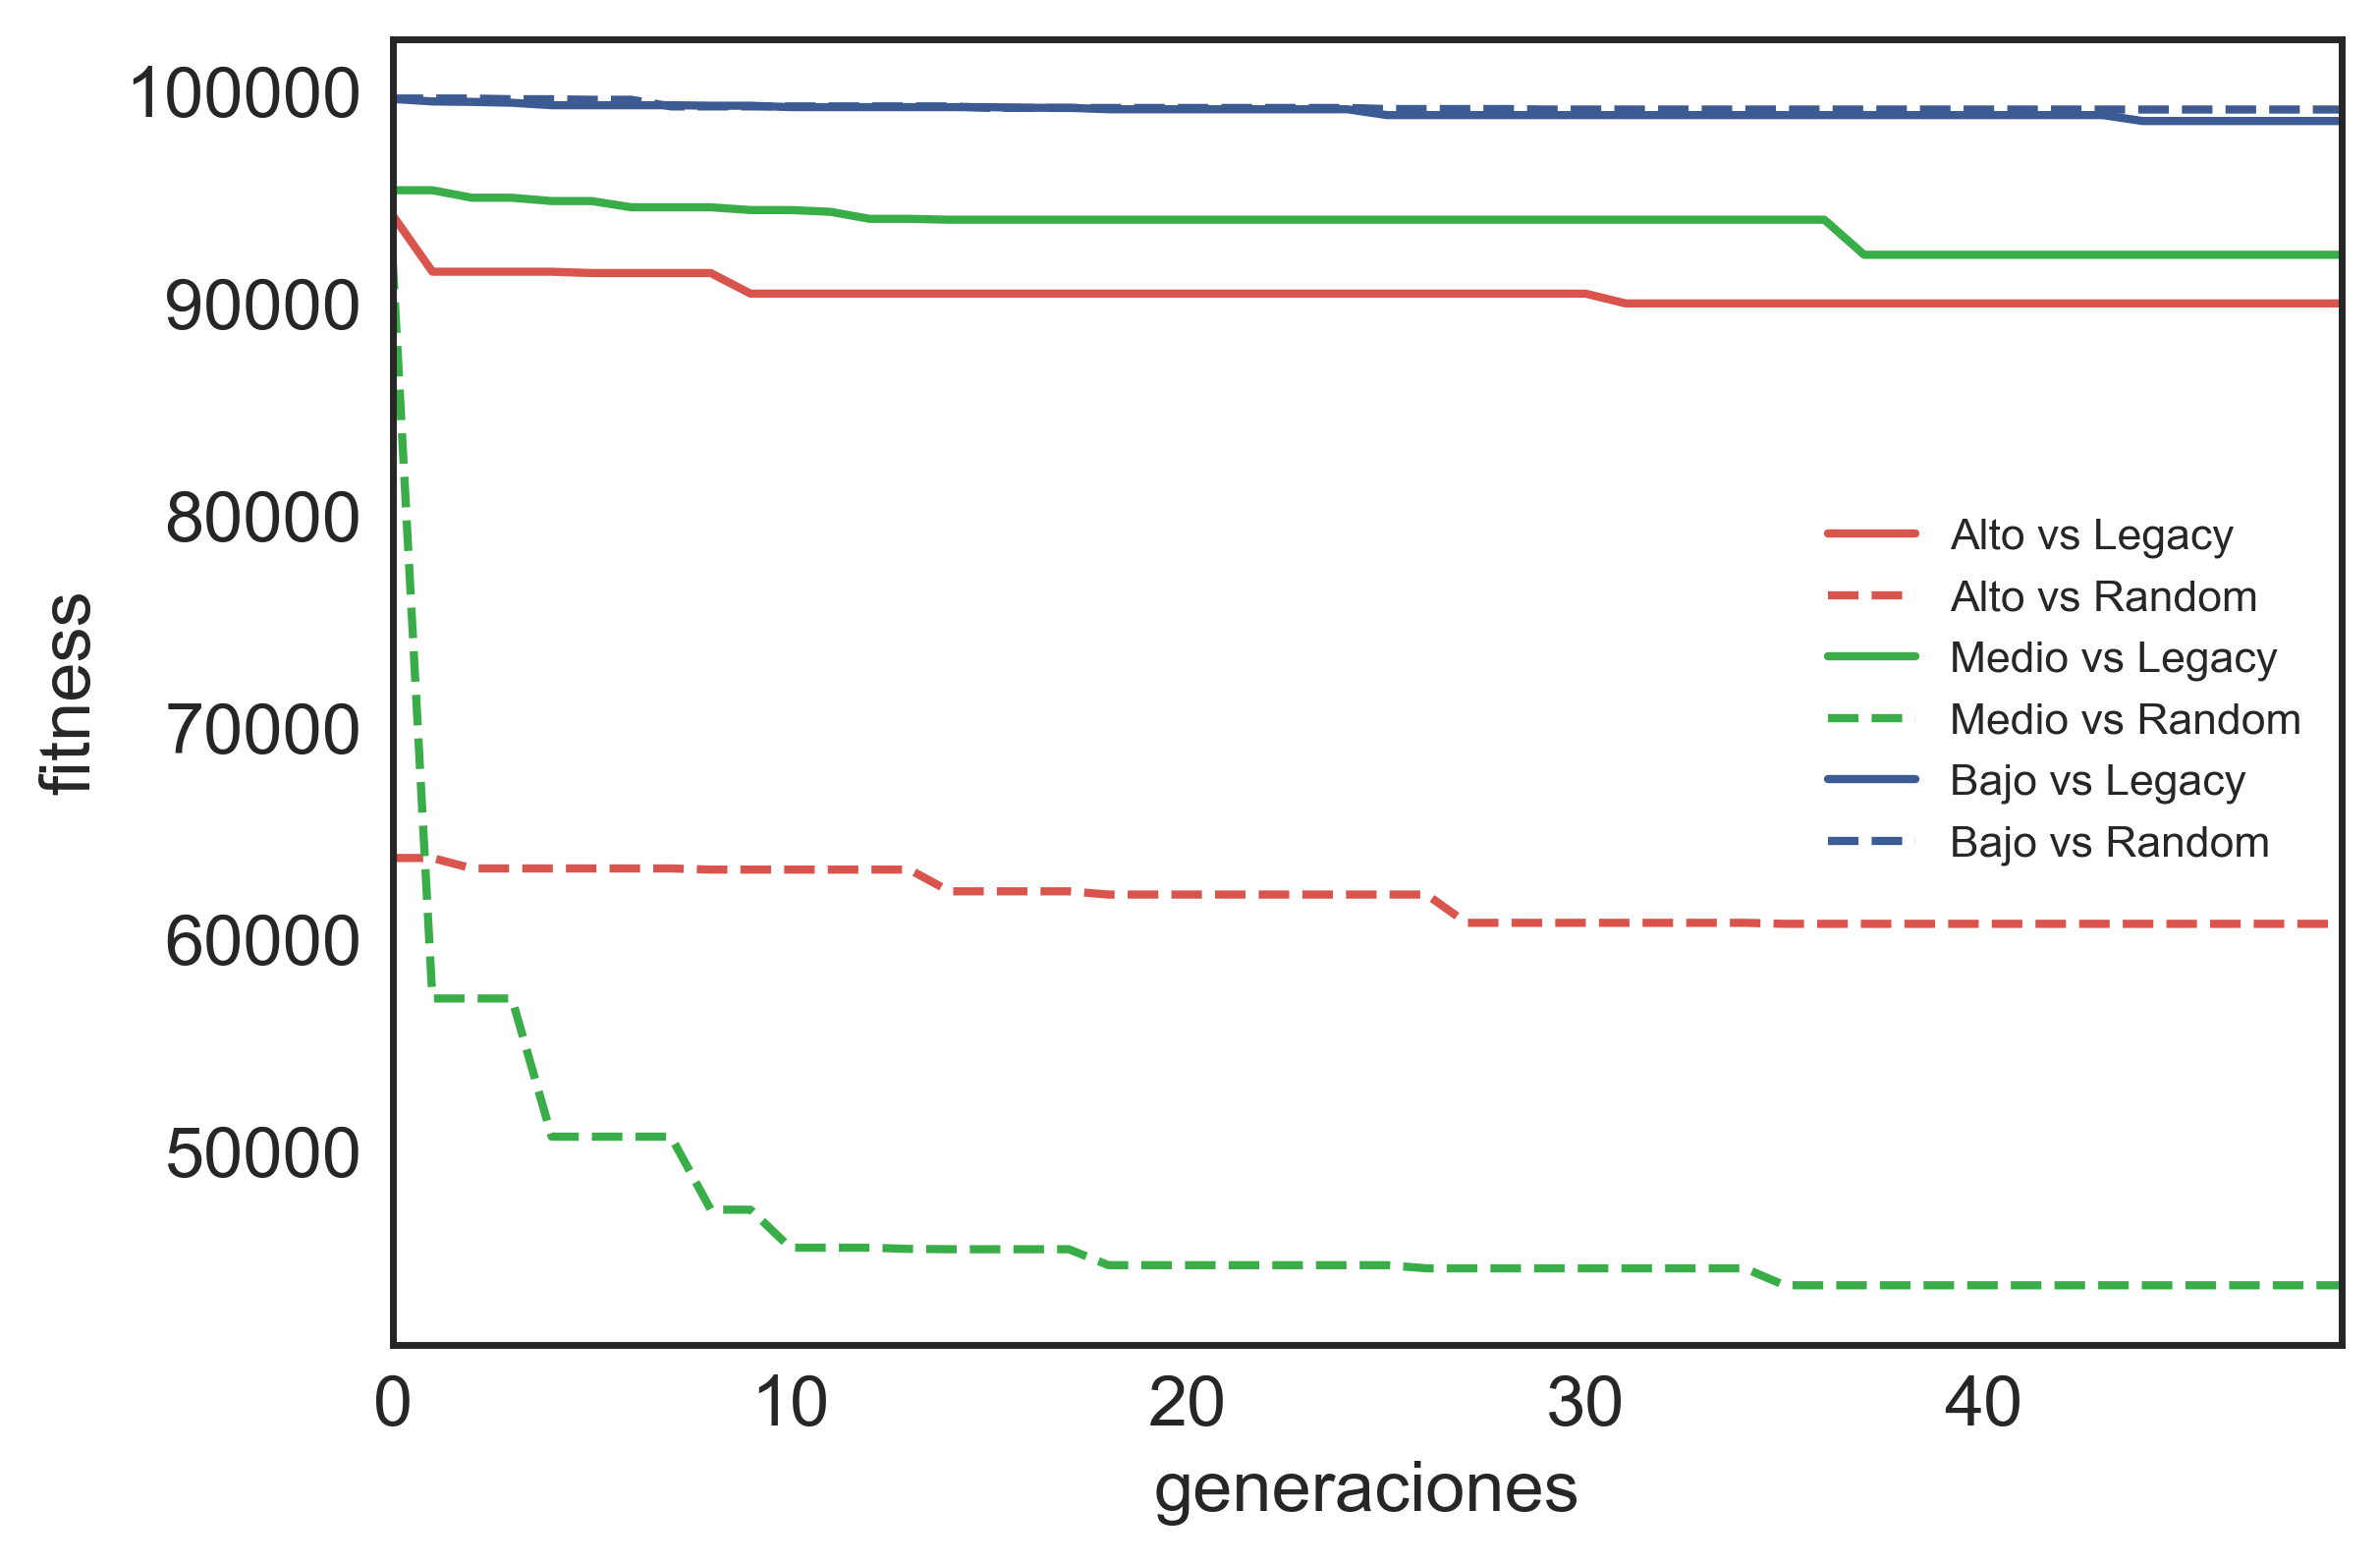
\includegraphics[width=0.8\textwidth]{grafica/all_fitnesses}
\label{grafica:comparacion-todas}
\caption{Gráfica de comparación de la evolución de una misma población usando las gramáticas de bajo, medio y alto nivel para dos controladores de fantasmas distintos (menos es mejor).}
\end{figure}
